% Appendix A

\chapter{User manual for the database application}
\label{AppendixA}
The source code for the application can be downloaded at \href{https://github.com/vietttifi/MasterThesisUiO}{\textbf{https://github.com/vietttifi/MasterThesisUiO}} and import to Android Studio in order to install the application to a Android device. The application has four main fragments as presented in Figure \ref{fig:AppendixA}, in which Sub figure\ref{fig:AppendixAa} is used to manage real time sources, Sub figure\ref{fig:AppendixAb} for importing EDF/EDF plus files, Sub figure \ref{fig:AppendixAc} for real time visualization, and Sub figure \ref{fig:AppendixAd} for database tasks and replay data from the database.
\begin{figure}
        \centering
        \subfigure[Real time]{\label{fig:AppendixAa}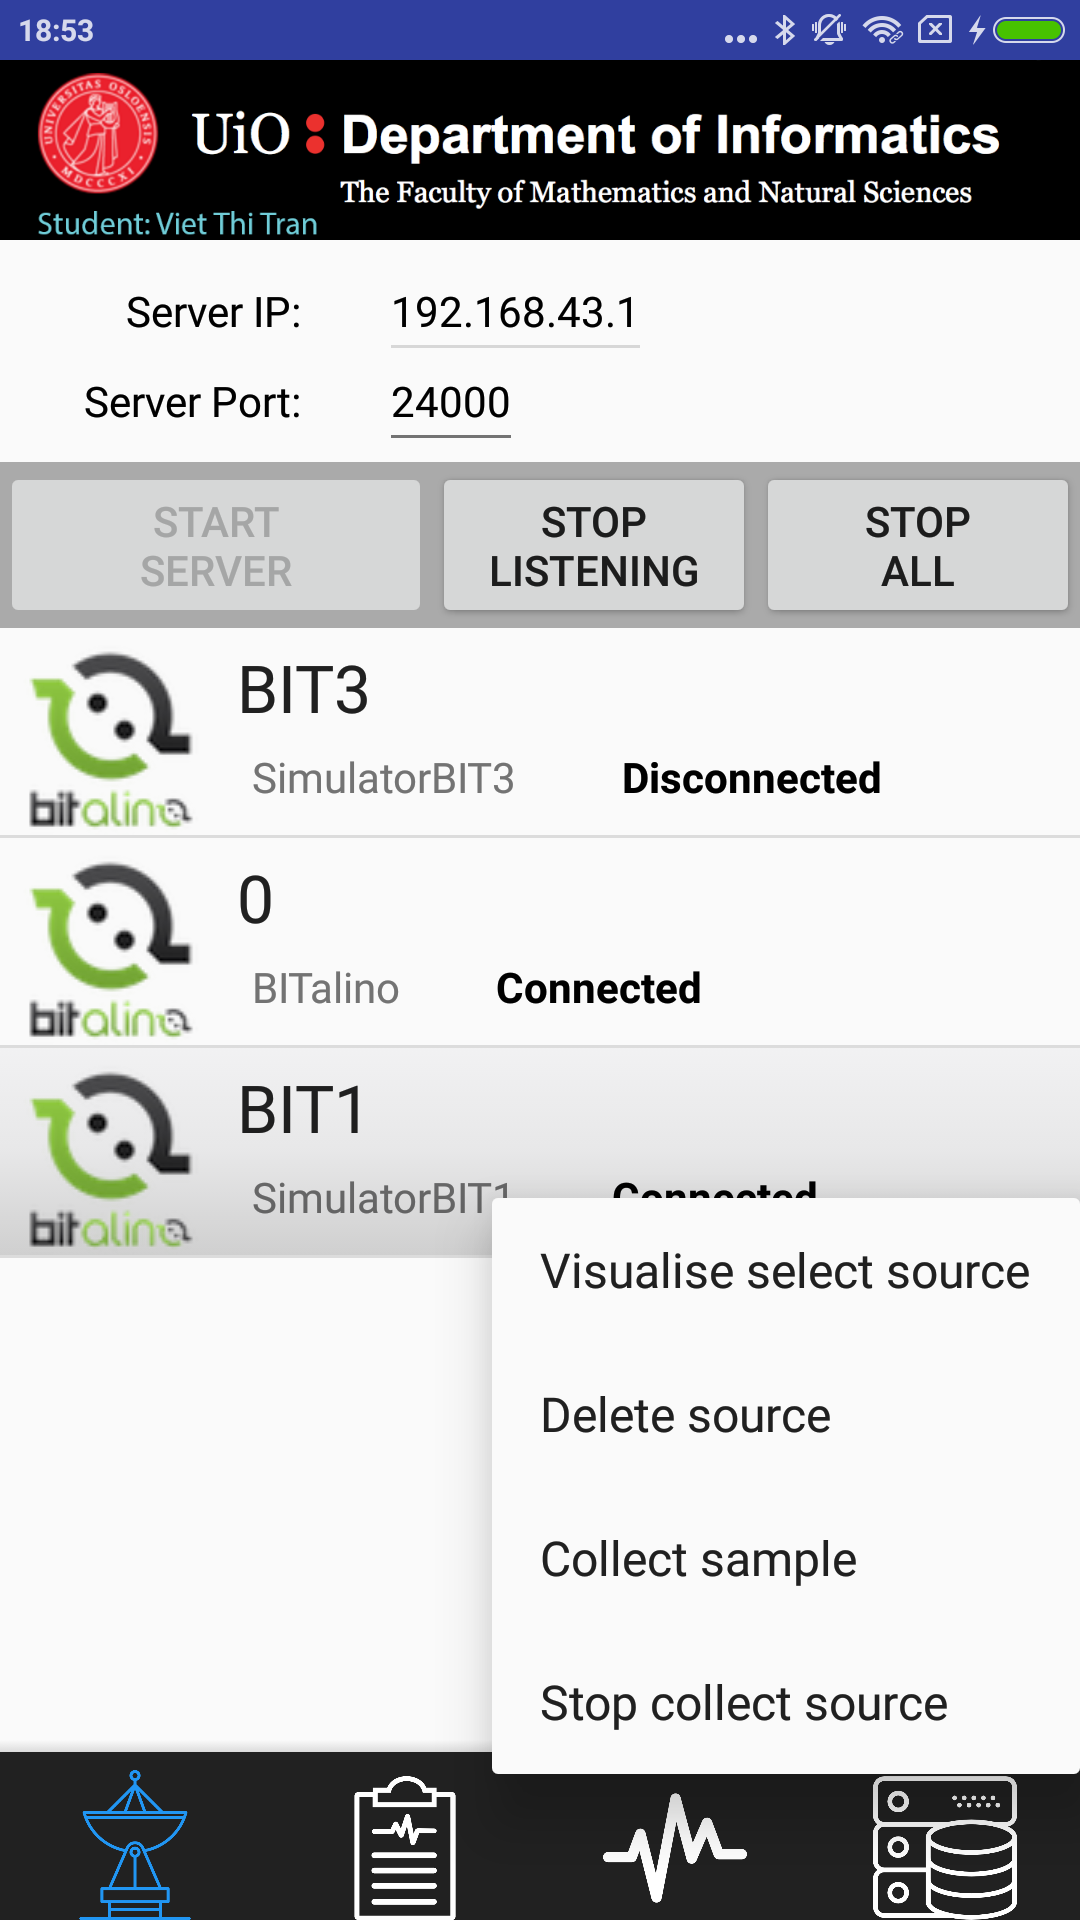
\includegraphics[width=50mm]{Figures/CESARGUIWrapper.png}}
        \subfigure[EDF import]{\label{fig:AppendixAb}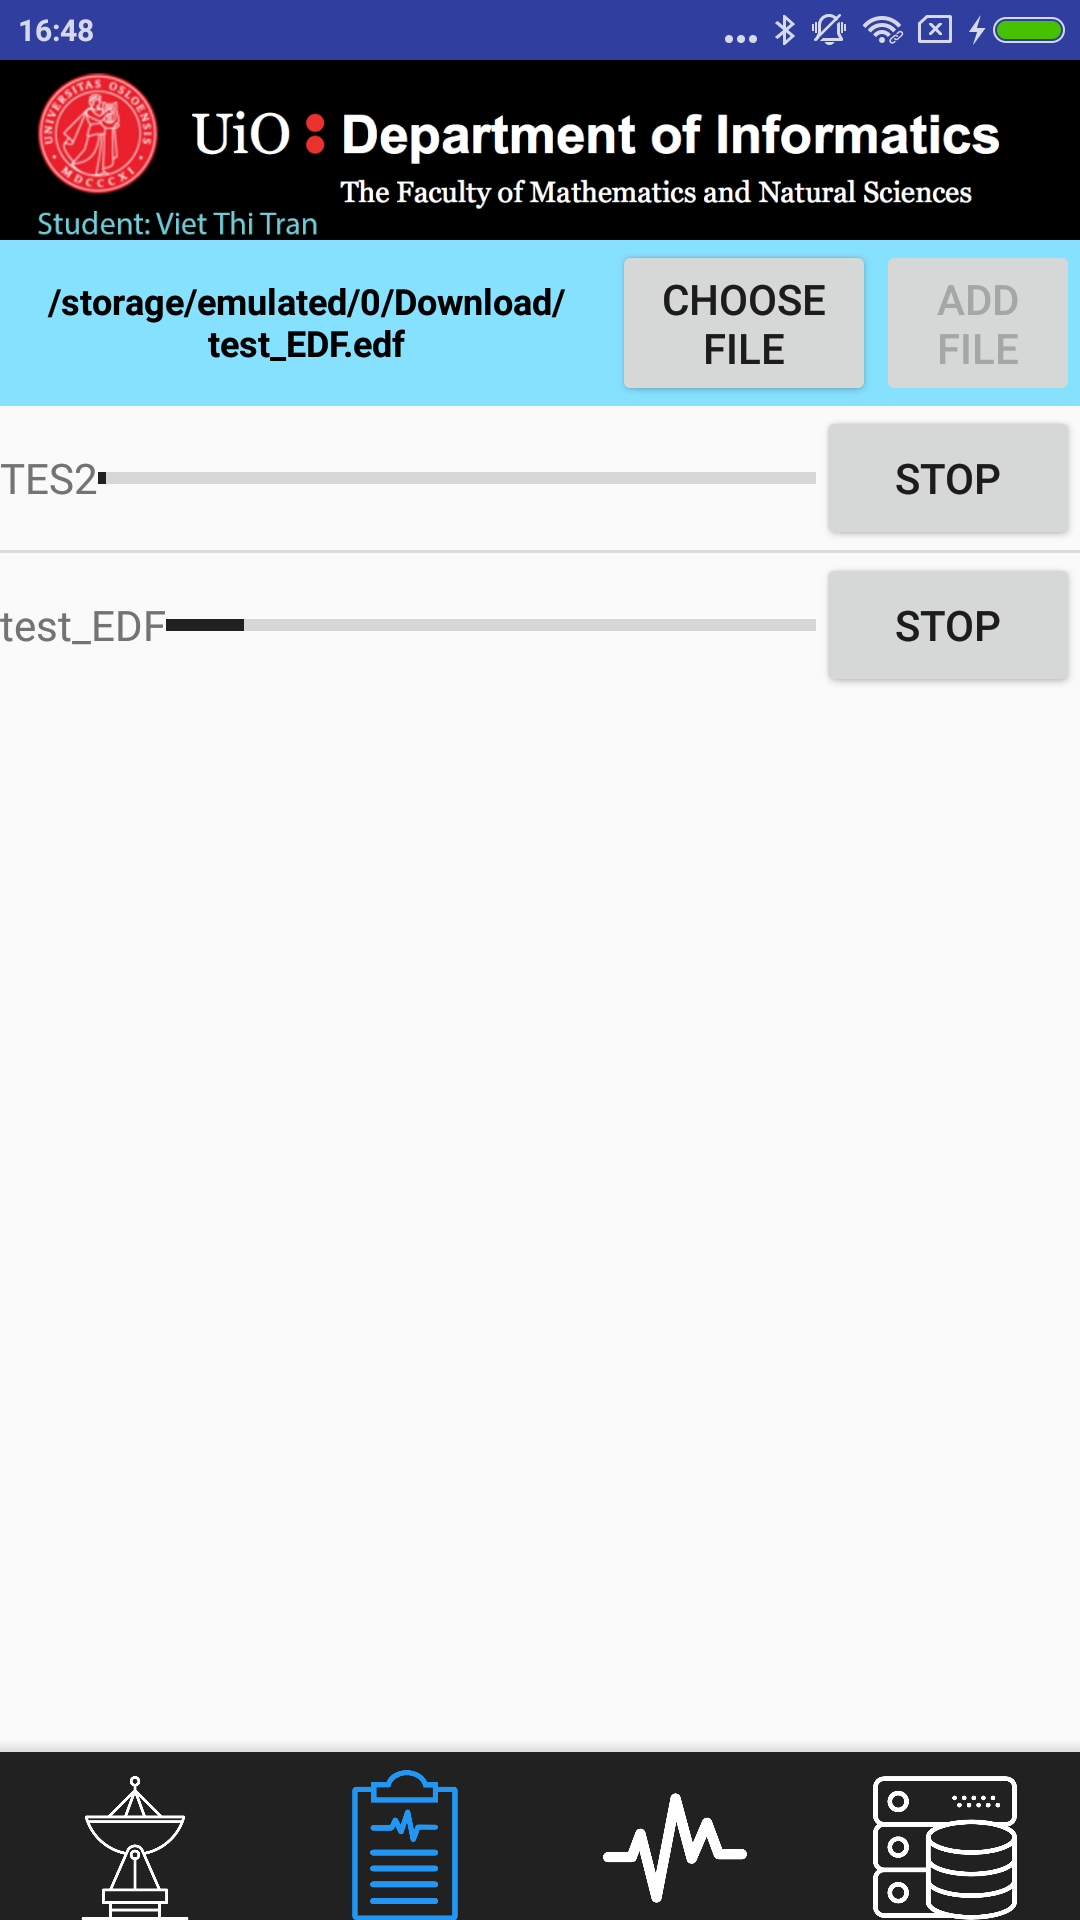
\includegraphics[width=50mm]{Figures/EDFimport.png}}
        \subfigure[EDF export]{\label{fig:AppendixAc}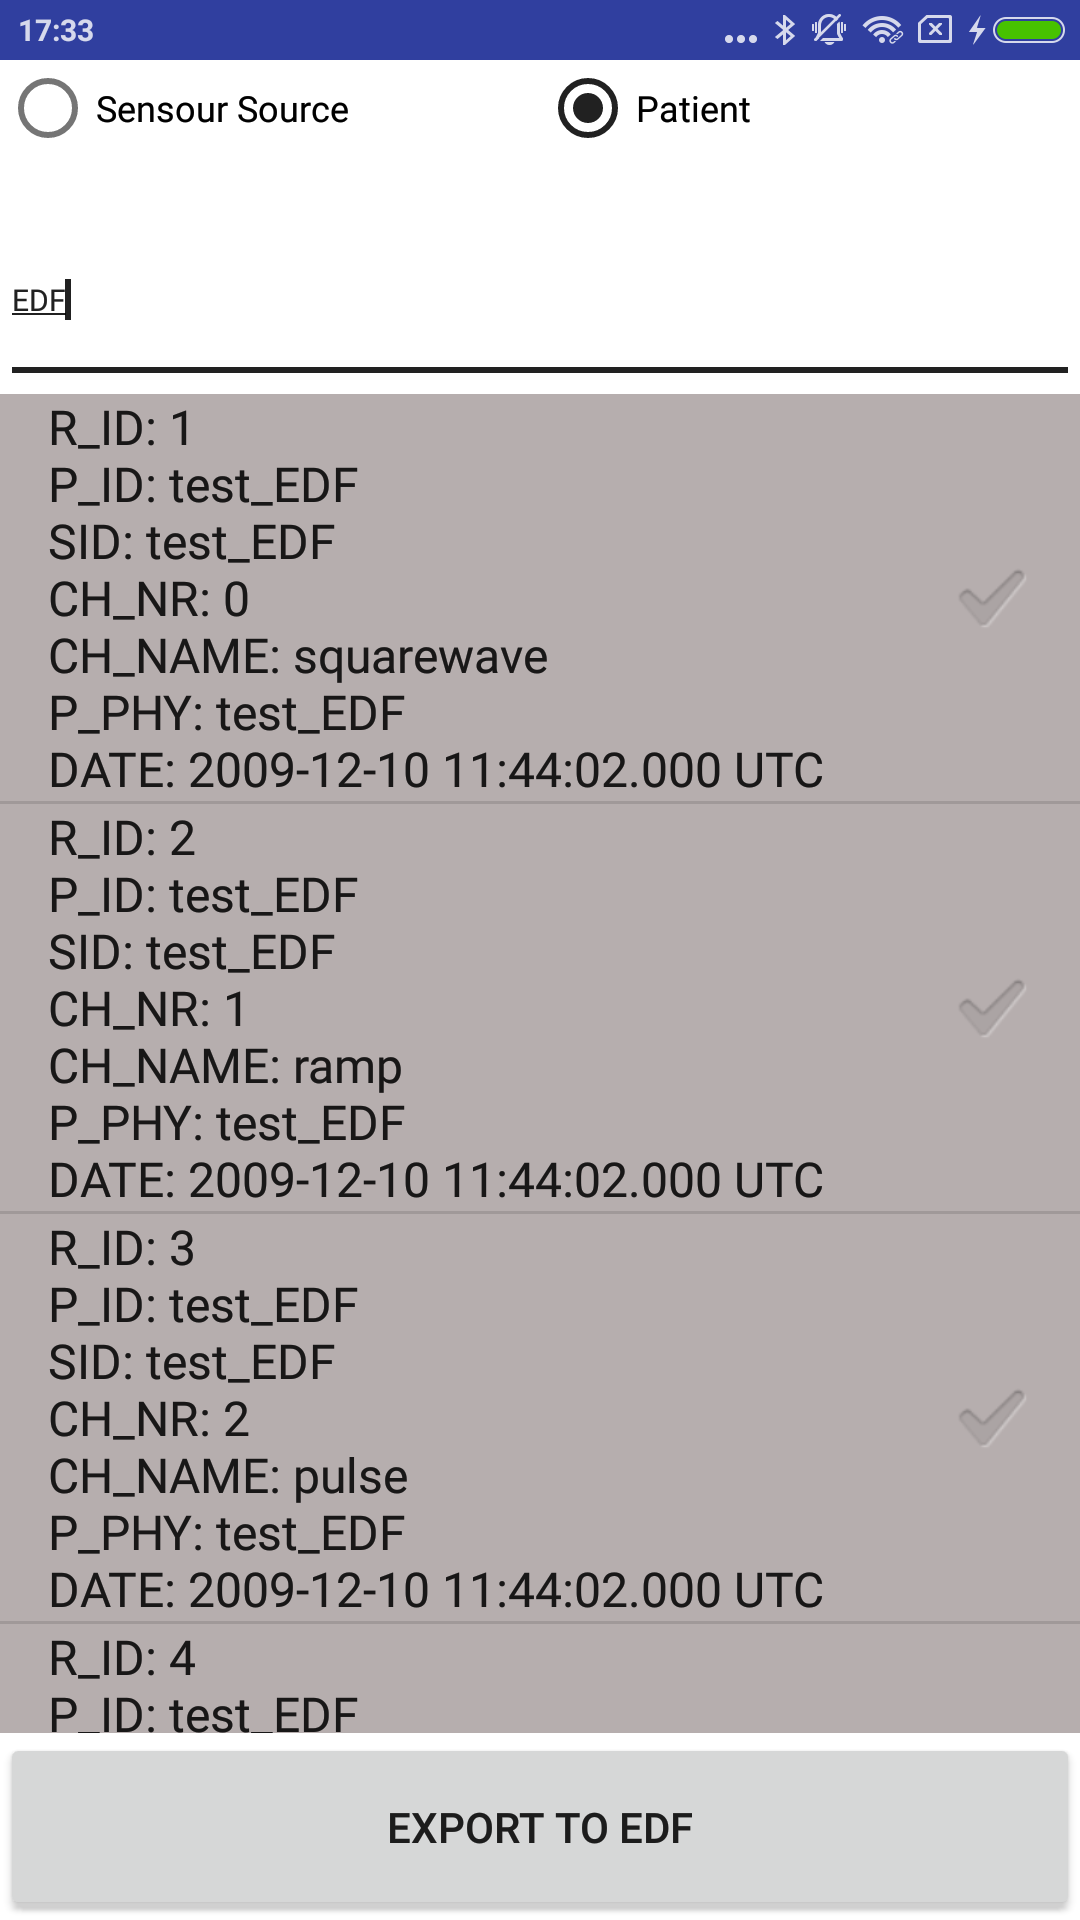
\includegraphics[width=50mm]{Figures/EDFexport.png}}
        \subfigure[Database tasks]{\label{fig:AppendixAd}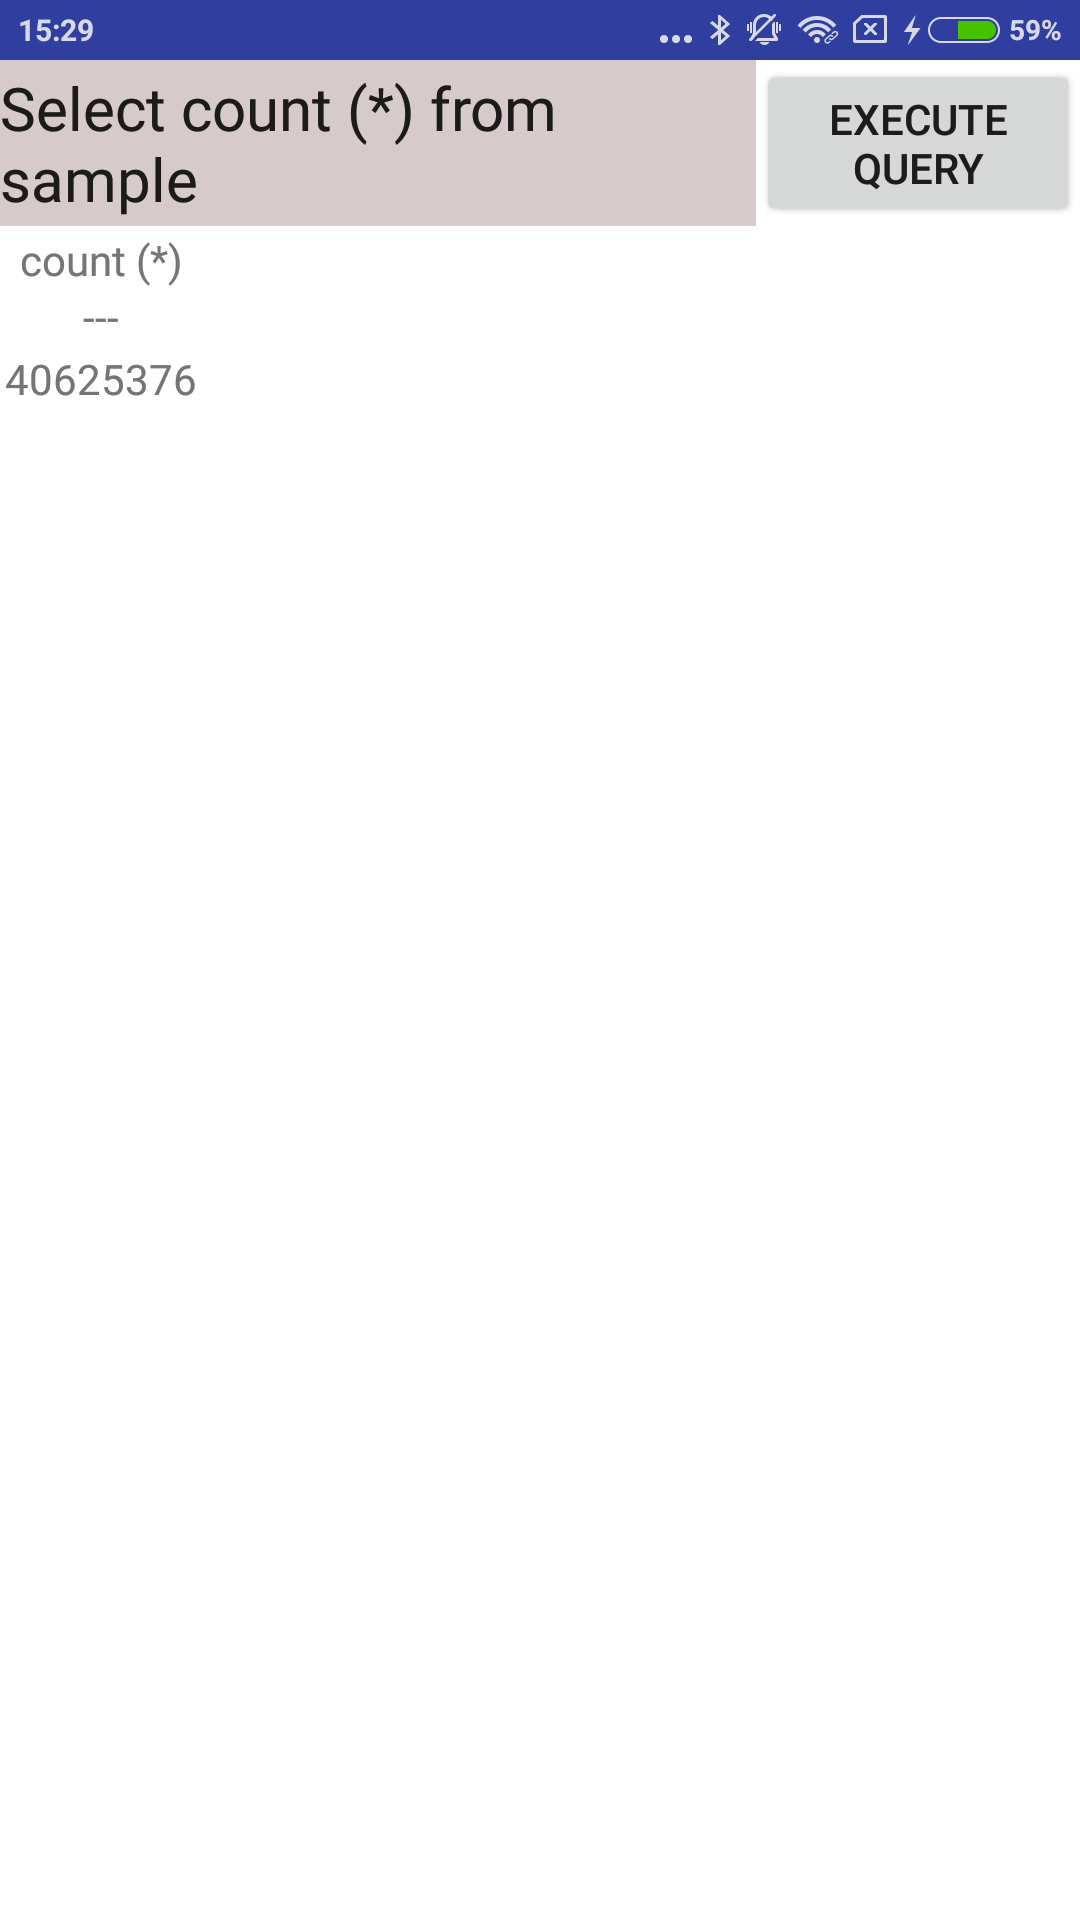
\includegraphics[width=50mm]{Figures/RawQuery.png}}
        \caption{Main fragments of the database application}
        \label{fig:AppendixA}
\end{figure}
\section{Real time wrapper}
As presented in Sub figure \ref{fig:AppendixAa}, the IP address and port number in which the device listens to are shown. Sensor sources can send data to the device by using the provided address. The port number is freely chosen, but not smaller than 1024. By long click on a source in the list, fours provided functions for the source are shown, which are visualization, source deletion, stop the collection, and begin a collection. Each source has a status which is either "connected", "storing", "plotting", "plotting and storing" or "disconnected" that presents a current status of the source. 
\section{Import EDF files}
A file chooser is presented after a user clicks on "choose file" button that lets the user choose a EDF/EDF plus file to read. By repeating "choose file" and "add file" actions, the user can simultaneously add multiple file. The user can stop the reading process by clicking on "stop" button.
\section{Visualize samples}
For real time sources, a user must choose a source from the source list of the real time fragment to visualize. The application currently supports mono-source visualization, but users can choose which channels in the source that they want to visualize.\\
For non real time sources, a user must query a record based on either patient, or sensor source information. By clicking on "apply" button, the user can play or pause the visualization. When pausing the visualization, the user can add and save annotations to the database. However, to save annotation is currently not supported in this thesis, because data analyses are not the main focus of the thesis, but it is not so difficult to implement. 
\section{Export EDF files}
Since data records are stored separately for each channel, by choosing data records that have the same patient, physician, and timestamp information, a full record for a patient at a specific time is retrieved. Users does not need to select all data records of the full record to export to a EDF/EDF plus file, they can select only the data records for specific interested channels to export.
\section{Raw query}
Users can execute their customized SQL queries by summiting the queries to the text box that presented in Sub figure \ref{fig:AppendixAd}. Since the application does not filter out the vulnerable queries such as DELETE or DROP TABLE, users must be responsible for the queries they submit to the application.
\section{BITalino simulator}
The simulator is found on in the project folder of the thesis on github.com at 